\appendix
\section{Technical appendix}
\label{sec:appendix}

\subsection{Comparison of neural network architecture}
\label{sec:appendixA}

\begin{table}
    \centering
\begin{tabular}{llll}
    \toprule
    architecture & top layer & \# neurons in top layer &       global accuracy \\
    \midrule
    EfficientNetB4 &   Flatten &                    128 &  0.663482 \\
    EfficientNetB4 &   Flatten &                    256 &  0.715764 \\
    EfficientNetB4 &   Flatten &                    512 &  0.697187 \\
    EfficientNetB4 &   GlobalAveragePooling2D &                    128 &  0.723726 \\
    EfficientNetB4 &   GlobalAveragePooling2D &                    256 &  0.715764 \\
    EfficientNetB4 &   GlobalAveragePooling2D &                    512 &  0.727972 \\
        ResnNet50 &   Flatten &                    128 &  0.481157 \\
        ResnNet50 &   Flatten &                    256 &  0.481423 \\
        ResnNet50 &   Flatten &                    512 &  0.522824 \\
        ResnNet50 &   GlobalAveragePooling2D &                    128 &  0.469745 \\
        ResnNet50 &   GlobalAveragePooling2D &                    256 &  0.469745 \\
        ResnNet50 &   GlobalAveragePooling2D &                    512 &  0.526274 \\
           VGG19 &   Flatten &                    128 &  0.708333 \\
           VGG19 &   Flatten &                    256 &  0.675425 \\
           VGG19 &   Flatten &                    512 &  0.692144 \\
           VGG19 &   GlobalAveragePooling2D &                    128 &   0.69931 \\
           VGG19 &   GlobalAveragePooling2D &                    256 &  0.678609 \\
           VGG19 &   GlobalAveragePooling2D &                    512 &   0.67224 \\
    \bottomrule
    \end{tabular}
\caption{\label{tab:app_nns}\footnotesize Comparison of global accuracy of different architectures of neural network
on a sample of data with signature types aggregated into three classes using the baseline image classification.
EfficientNetB4 with GlobalAveragePooling2D and 256 neurons has been used in the final experiment.}
\end{table}


\pagebreak

\subsection{Within-class performance by spatial signature}
\label{sec:appendixB}

\begin{figure}
    \centering
    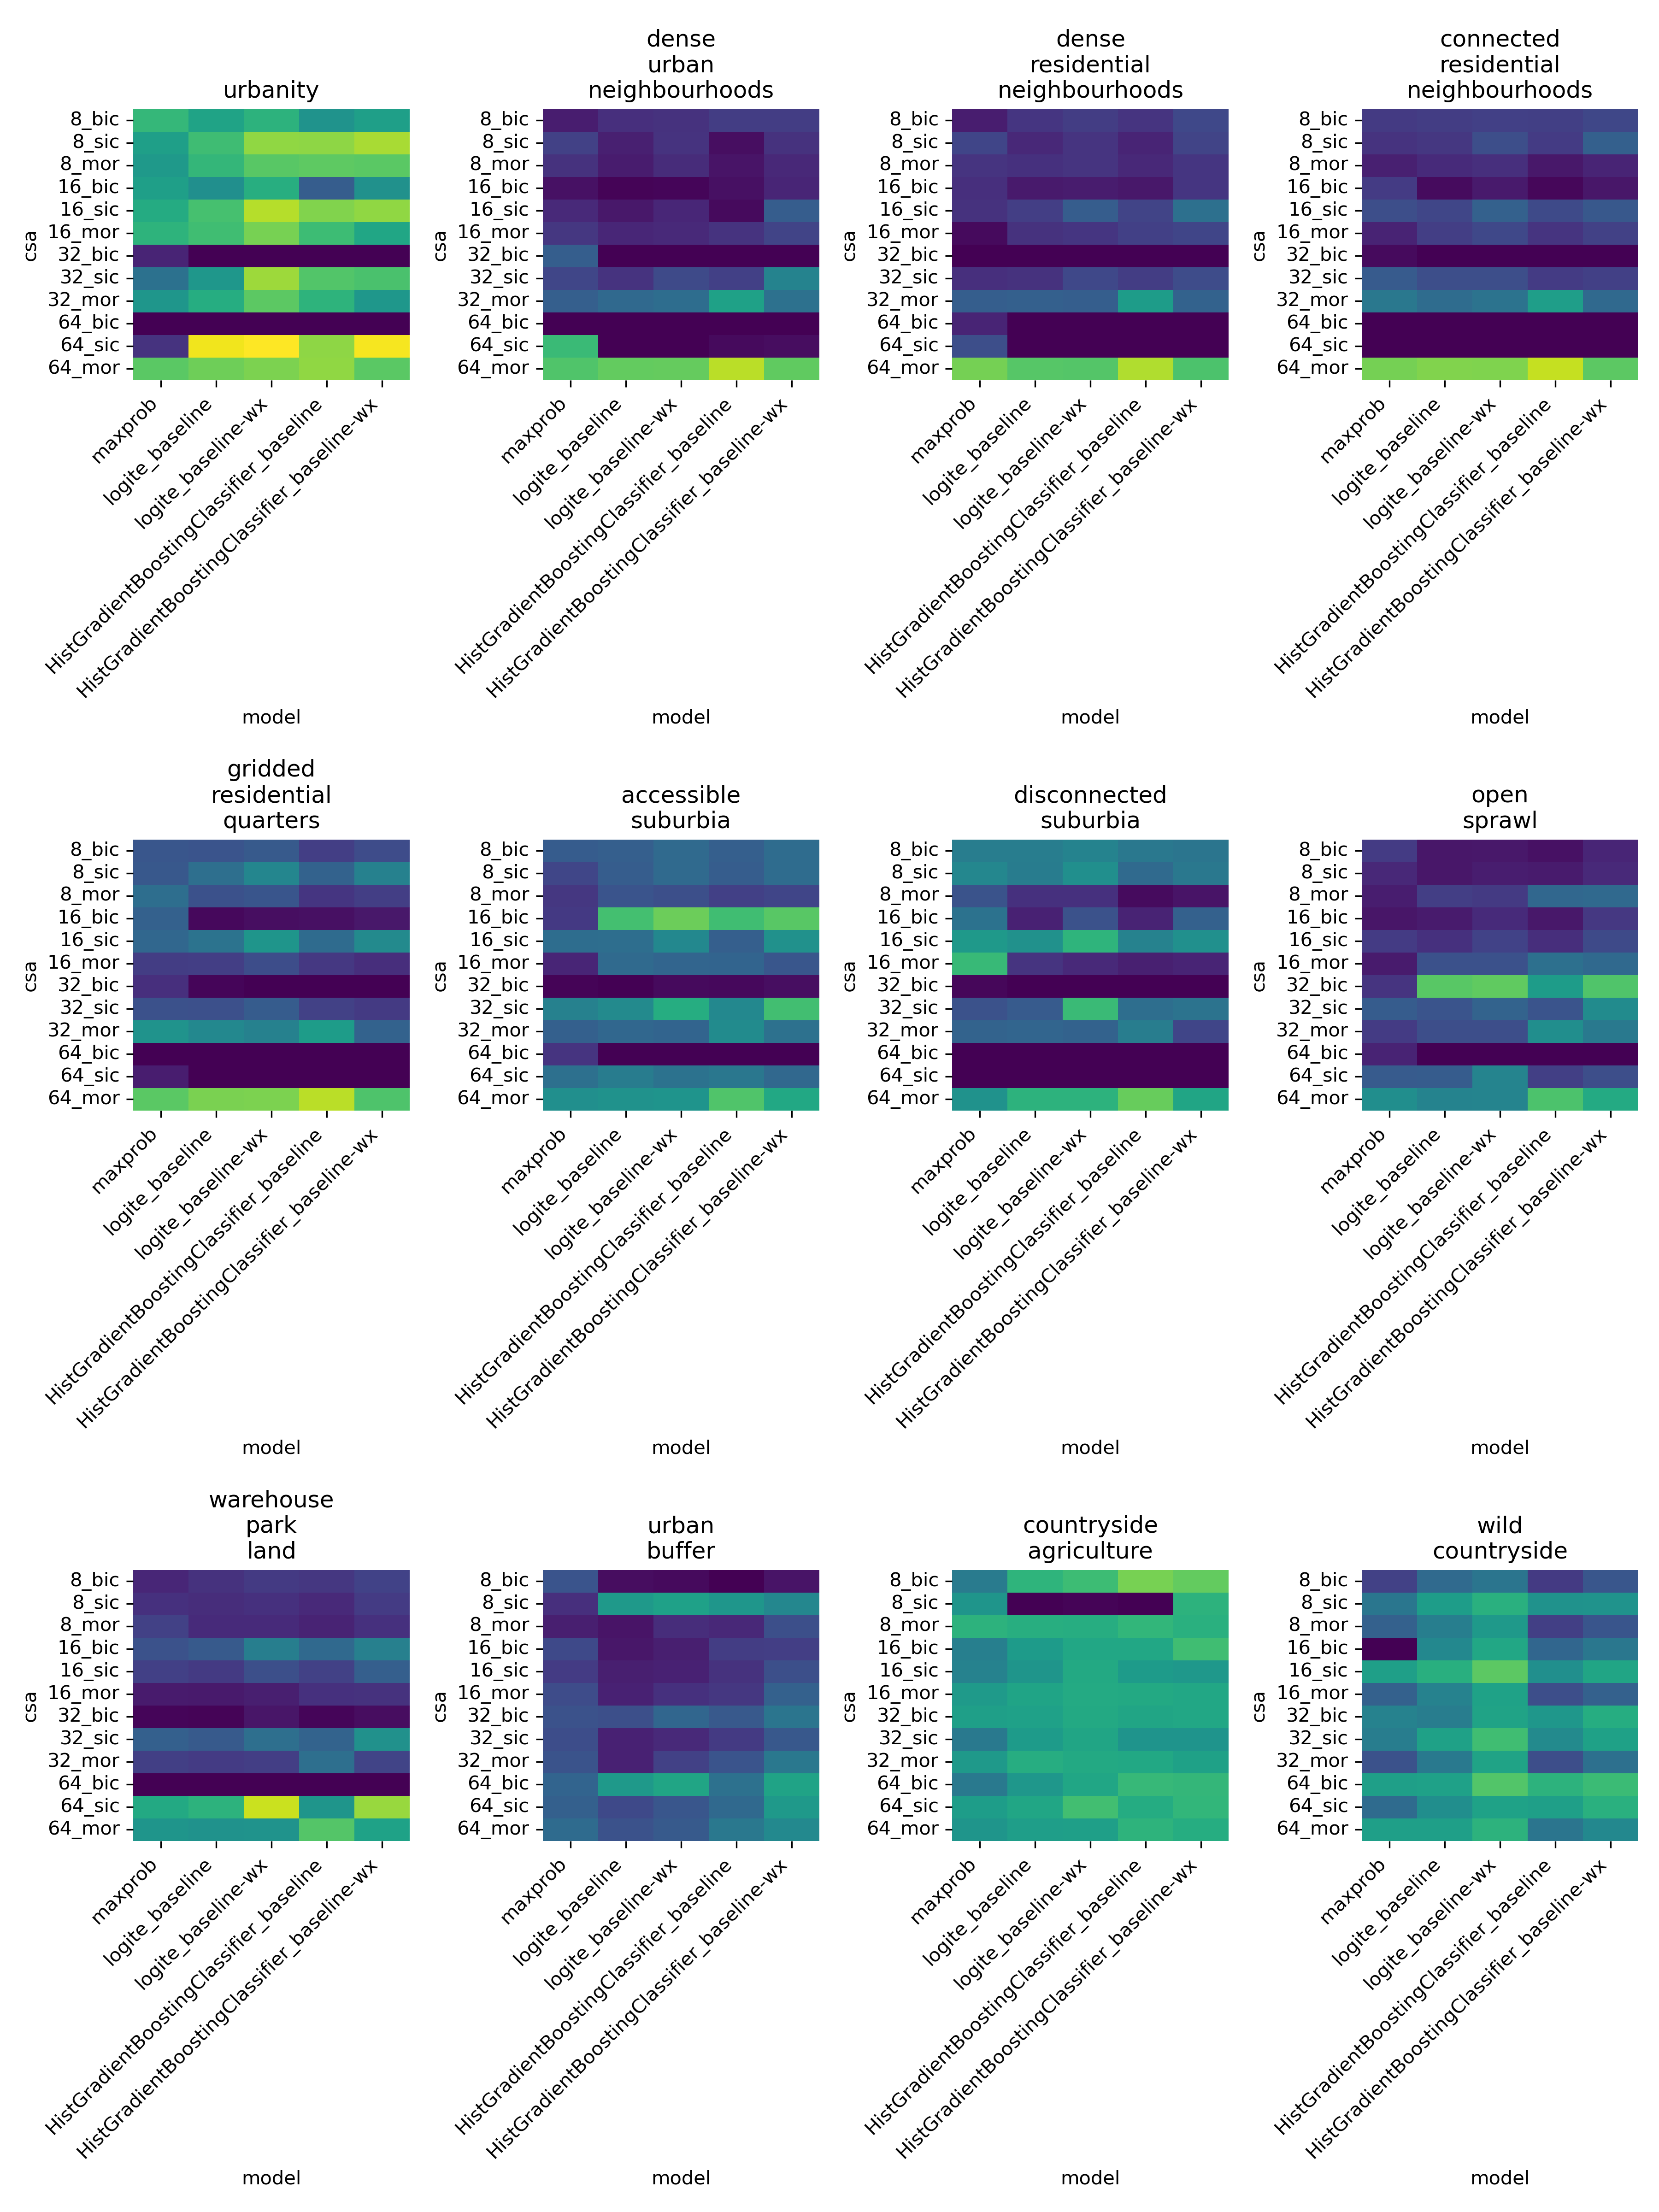
\includegraphics[width=0.8\linewidth]{fig/wc_accuracy_x_signature.png}
    \caption{\footnotesize Within-class accuracy scores grouped by signature. Each panel
    represents results from one of the 12 signatures predicted. Each column in
    the heatmap
    corresponds to one of the five models compared, namely:
    histogram-based boosted classifier (\texttt{HGBC}) with features
    pertaining only to a given chip (\texttt{baseline}) or including also features
    from neighbouring ones (\texttt{baseline-wx}); Logit ensemble
    (\texttt{logite}) with the same two variations; and a simpler maximum
    probability approach (\texttt{maxprob}). Each row
    corresponds to a pair of chipsize (8, 16, 32, and 64 pixels)
    and architecture (baseline image classification, or \texttt{bic}; sliding
            image classification, or \texttt{sic}; and multi-output
    regression, or \texttt{mor}) used in the neural network stage of the
    pipeline.}
    \label{fig:wc_accuracy_x_signature}
\end{figure}

\pagebreak

\subsection{Confusion matrices}
\label{sec:appendixC}
